\label{relative_performance}
In Section \ref{section2C}, we show the importance of incorporating characteristics in explaining the returns of mutual funds. The results in the previous section demonstrate an important flaw of the traditional factor model alphas, insofar as they attribute skill to passive exposures to characteristics. Therefore, we propose a mutual fund performance measure which adjusts performance for exposures to both factor betas and characteristics. 

In this section, we examine the extent to which our new double-adjusted alpha affects inference relating to relative mutual fund performance. We replicate the work of several mutual fund performance studies using  six-factor alpha as our baseline measure of performance, computed  using the traditional time series regression approach.\footnote{Even though the hierarchical Bayes model also provides estimates of fund alphas, we choose the time series regression approach as this is standard in previous literature. Moreover, the Bayesian estimate of standard alpha makes use of cross-sectional information. To highlight the difference made by adjusting performance for characteristics, we compare our double-adjusted alpha to a performance measure which is not influenced by these characteristics.} Because we use traditional alpha as our baseline performance measure, we can  easily extend previous analysis with the two components of alpha, our double-adjusted measure and the portion of alpha associated with characteristics (see Eqs.(\ref{double_adjusted_alpha}) and (\ref{char})). The decomposition of alpha will indicate the extent to which both components contribute to the main findings of previous studies.\footnote{We follow \citet{busse2017double} in reassessing previous findings in the mutual fund literature using the double-adjusted performance measure. In addition to the analyses in this paper, they also reevaluated the relation between fund performance and the industry concentration \citep{kacperczyk2005industry}, the return gap \citep{kacperczyk2008unobserved}, and active share \citep{cremers2009active}.  } 

We begin by calculating the difference in fund percentile performance rankings between using double-adjusted alpha in comparison to those based on alpha. Next, central to the mutual fund performance literature are studies that analyze persistence in fund performance, e.g., \citet{carhart1997persistence}. Other studies examine the relation between fund performance and certain fund features, such as a fund's factor model R-squared \citep{amihud2013mutual} and a fund's investors cash flows \citep{barber2016factors}. We plug in our estimates of the posterior mean of both components of alpha in the analysis of these papers. We use the estimation methods used in these papers to accommodate a fair comparison between inferences based on traditional alpha and those based on double-adjusted alpha.

\subsection{Relative Mutual Fund Performance Rankings}
We examine the degree to which our new performance measure alters the performance rankings of funds. In each month in our sample, we sort funds into percentiles based on six-factor alpha ($\alpha$) and on double-adjusted six-factor alpha ($\alpha^*$). Given a number of $N_t$ funds in month $t$, we obtain pairs of percentile ranks for each fund $\{(P^{\alpha}_{1t},P^{\alpha^*}_{1t}),..., (P^{\alpha}_{N_tt},P^{\alpha^*}_{N_tt})\}$. Using the percentile rank pairs we compute Kendall's tau coefficient, which is a correlation coefficient between two rankings. We find a time series average of Kendall's tau equal to 0.70, which indicates differences between the two rankings. 

To examine the impact of double-adjusted alpha on performance rankings in more detail, we compute the difference between the performance ranks $P^{\alpha}_t$ and $P^{\alpha^*}_t$ for each fund in each month $t$. Table \ref{table5}
presents the time series average distribution (across all months in our sample) of the difference in percentile performance rankings. We find that the median change in percentile rankings is roughly 9\%, i.e., a fund which is ranked in the median percentile according to alpha is ranked in either the 41th or 59th percentile based on double-adjusted alpha. Moreover, many funds exhibit dramatic changes in percentile ranking, with 10 (5) percent of funds exhibiting a mean change in percentile ranking of at least 22.99\% (27.24\%). Thus, we find that adjusting traditional alpha for characteristics materially impacts the performance ranking of funds.

% \begin{singlespacing}
% \begin{table}[H]
% \small
% \centering
% \setlength{\tabcolsep}{12.5pt}
% {\captionsetup{justification=centering,singlelinecheck=off}
% \caption{\bfseries Change in performance percentile rankings  }}
% \caption*{This table presents the differences between the performance percentile ranks based on double-adjusted six-factor alpha ($\alpha^*$) relative to six-factor alpha ($\alpha$). These performance measures are calculated using rolling windows with a window size of 24 months (see section \ref{double_alpha}). Each month in our sample period we compute the difference between the percentile ranking based on alpha ($P^\alpha$) and the percentile ranking based on double-adjusted alpha ($P^{\alpha^*}$). We report the time series average distribution of the difference between performance rankings. The sample period is February 2001 to December 2016.}
% {\captionsetup{justification=centering,singlelinecheck=off}

% \label{my-label}
% \begin{tabular}{crrrrrrr}
% \hline
% Percentile     & 5      & 10     & 25    & 50   & 75    & 90    & 95    \\ \hline
% Rank (\%)   &  -22.93 & -17.89 &	-8.99 &	-0.02 &	9.05 & 17.84 &	23.07 \\
% Abs. Rank (\%) & 0.99 & 	1.49 & 	4.08 &	9.03 &	15.98 & 	22.99 &	27.24\\ \hline
% \end{tabular}
% \end{table}
% \end{singlespacing}

\subsection{Mutual Fund Return Persistence}
Mutual fund persistence is well documented in the finance literature. Early works include \citet{grinblatt1992persistence}, \citet{brown1995performance} and \citet{wermers1997momentum}, which document significant persistence in mutual fund rankings based on returns after adjustment for risk. This persistence lasts over horizons of one to three years, and they attribute the persistence to ``hot hands" or common investment strategies. \citet{carhart1997persistence} add stock momentum as an additional risk factor and find a significant difference in abnormal returns of more than 4\% on an annual basis. Drawing on Carhart's findings, \citet{bollen2004short} find an average abnormal return of 39 basis points for the top quintile in the post-ranking quarter. This post-ranking abnormal return disappears when evaluated over longer periods. 

We examine return persistence in several performance measures: six-factor alpha ($\alpha$), double-adjusted six-factor alpha ($\alpha^*)$ and characteristic-driven performance ($\alpha^{char}$). If our new performance measure, which accounts for characteristics, is a better indicator of true skill, we expect double-adjusted alpha to account for most of the persistence in alpha, such that double-adjusted alpha persists for a longer period. In this case, there should be no distinct return pattern using characteristic-driven performance. That is, if true skill goes beyond the premiums which are passively associated with characteristics. 

We replicate the studies on return persistence.\footnote{This paper adopts a similar approach to the one used in \citet{carhart1997persistence}. The only difference is the frequency of rebalancing, which is set to a quarterly basis in this work. \citet{busse2017double} analyzed persistence in their double-adjusted performance measure. They adopt an annual rebalancing of portfolios and found new evidence of persistence in mutual fund skill based on their double-adjusted performance measure.} Each quarter-end, we sort funds into deciles using the aforementioned performance measures; decile 10 contains the best performing funds and decile 1 contains the worst performing funds. We hold the sorted portfolios for up to six years and compute the equal-weighted return in each decile in the post-ranking period. To deal with overlapping decile portfolios formed in different quarters, we compute the equal-weighted return across overlapping periods. We examine the post-ranking performance by concatenating the returns of all post-ranking periods for each decile and estimate six-factor alpha using the resulting time series of post-ranking (monthly) returns for each decile. 

Table \ref{table6} presents the persistence results. Panel A shows strong evidence of persistence in standard six-factor alpha. In the short term, the average difference in alpha between the top and bottom deciles is 0.28 (t = 3.62) in the following quarter and 0.27 (t = 3.85) in the year thereafter, both of which significant from a statistical and an economic perspective. This abnormal return difference remains statistically significant in the second and third year after formation, followed by a decrease in the top-minus-bottom post ranking abnormal return from the fourth year onwards. Consistent with the findings of \citet{carhart1997persistence}, we find that the majority of the return spread is driven by past losing funds in the bottom deciles. In untabulated results, we find significant negative alphas in the bottom decile with t-statistics below -3. 

The results in Panel B show strong evidence that the double-adjusted six-factor alpha predicts future fund performance. We find a distinct return pattern across deciles sorted on our double-adjusted performance measure, as post-ranking alpha increases nearly monotonically across deciles and indicates a sizable return spread of 0.19 (t = 5.31) in the post-ranking quarter. The top-minus-bottom portfolios yield statistical significant alphas between 0.05 and 0.17, which persist up to six years. In Figure \ref{figure2}, we analyze return persistence on the long term. We graph the cumulative six-factor alpha of the top-minus-bottom portfolios, where the three plots lines represent alternative sorts on six-factor alpha, double-adjusted six-factor alpha, and characteristic-driven performance. The plots indicate an upward trend in the cumulative performance of both alpha and double-adjusted alpha, which lasts for the entire holding period of ten years. The results in Panel B of Table \ref{table6} combined with the plots from Figure \ref{figure2} suggest that double-adjusted alpha reflects true skill, which pays off in the long run such that persistence in this component of alpha causes most of the persistence in alpha. Our results are in line with the persistence analysis in \citet{busse2017double}. Using their double-ajdusted alpha they find evidence of persistence in fund four-factor alphas up to nine years after the initial ranking. We show that persistence is also present when a shorter sample period is used. 

In Panel C of Table \ref{table6} we turn to the component of alpha driven by passively loading on characteristics. The average return difference in alpha in the first year after formation is 0.16 with insignificant t-statistics, followed by a slight reversal from the second year onwards. The graph in Figure \ref{figure2} shows that sorts on characteristic-driven performance does not exhibit a distinct return pattern after formation in the long term. These results indicate that returns associated with characteristics do not convey information about future fund performance. This supports the claim that evidence of return predictability in alpha is mostly accounted for by the component adjusted for passive loadings on characteristics. By removing this noisy component, which does not detect skill, double-adjusted alpha is a more precise measurement of skill, leading to stronger evidence of persistence in mutual fund performance. 


% \begin{singlespacing}
% \begin{table}[h!]
% \small
% {\captionsetup{justification=centering,singlelinecheck=off}
% \caption{ \bfseries Mutual fund performance persistence }}
% \caption*{This table presents returns of decile porfolios sorted by six-factor alpha (Panel A), double-adjusted six-factor alpha (Panel B) and characteristic-driven performance (Panel C). These performance measured are calculated using rolling windows with a window size of 24 months. Portfolios are rebalanced every quarter-end and are held for up to six years. To deal with overlapping portfolios, we follow \citet{jegadeesh1993returns} to take the equal-weighted return across overlapping portfolios formed in different quarters. Two different returns are reported: the excess return over the risk-free rate and the Fama-French six-factor alpha. T-statistics, shown in parenthesis, are computed using White's standard errors. Estimated significant at the 5\% level are in bold font. The sample period is May 1980 to December 2015.}
% \label{my-label}
% \begin{tabular}{crrrrrrrrrrr}
% \hline
%       & \multicolumn{2}{c}{Qtr 1}     &  & \multicolumn{2}{c}{Qtr 1-4}   &  & \multicolumn{2}{c}{Qtr 5-12}  &  & \multicolumn{2}{c}{Qrt 13-24} \\ \cline{2-3} \cline{5-6} \cline{8-9} \cline{11-12} 
% Decile & Excess        & 6F alpha      &  & Excess        & 6F alpha      &  & Excess        & 6F alpha      &  & Excess       & 6F alpha       \\ \hline
% \multicolumn{12}{l}{Panel A: Six-factor alpha}                                                                                                         \\
% 1      & 0.53          & -0.17         &  & 0.54          & -0.17         &  & 0.55          & -0.12         &  & 0.51         & -0.12          \\
% 2      & 0.56          & -0.08         &  & 0.56          & -0.09         &  & 0.55          & -0.10         &  & 0.55         & -0.07          \\
% 3      & 0.56          & -0.08         &  & 0.56          & -0.08         &  & 0.56          & -0.08         &  & 0.53         & -0.09          \\
% 4      & 0.56          & -0.08         &  & 0.56          & -0.08         &  & 0.57          & -0.07         &  & 0.52         & -0.09          \\
% 5      & 0.57          & -0.07         &  & 0.57          & -0.07         &  & 0.55          & -0.08         &  & 0.52         & -0.09          \\
% 6      & 0.57          & -0.06         &  & 0.56          & -0.06         &  & 0.53          & -0.09         &  & 0.53         & -0.08          \\
% 7      & 0.58          & -0.05         &  & 0.58          & -0.05         &  & 0.55          & -0.07         &  & 0.52         & -0.09          \\
% 8      & 0.59          & -0.05         &  & 0.58          & -0.06         &  & 0.55          & -0.08         &  & 0.52         & -0.08          \\
% 9      & 0.64          & -0.01         &  & 0.63          & -0.01         &  & 0.57          & -0.05         &  & 0.53         & -0.08          \\
% 10     & 0.68          & 0.01          &  & 0.66          & 0.00          &  & 0.60          & -0.04         &  & 0.55         & -0.08          \\
% 10-1  & 0.16          & 0.18          &  & 0.13          & 0.17          &  & 0.05          & 0.09          &  & 0.04         & 0.04           \\
%       & (\textbf{2.93}) & (\textbf{3.45}) &  & (\textbf{2.51}) & (\textbf{3.59}) &  & (1.16)          & (1.85)          &  & (1.19)         & (1.18)           \\
%       &               &               &  &               &               &  &               &               &  &              &                \\
% \multicolumn{12}{l}{Panel B: Double-adjusted six-factor alpha}                                                                                 \\
% 1      & 0.55          & -0.15         &  & 0.56          & -0.14         &  & 0.54          & -0.13         &  & 0.50         & -0.13          \\
% 2      & 0.57          & -0.09         &  & 0.55          & -0.11         &  & 0.55          & -0.10         &  & 0.52         & -0.10          \\
% 3      & 0.58          & -0.07         &  & 0.59          & -0.06         &  & 0.55          & -0.10         &  & 0.53         & -0.08          \\
% 4      & 0.55          & -0.08         &  & 0.57          & -0.07         &  & 0.56          & -0.07         &  & 0.51         & -0.10          \\
% 5      & 0.59          & -0.04         &  & 0.57          & -0.06         &  & 0.55          & -0.08         &  & 0.52         & -0.09          \\
% 6      & 0.56          & -0.06         &  & 0.55          & -0.07         &  & 0.54          & -0.08         &  & 0.52         & -0.09          \\
% 7      & 0.58          & -0.06         &  & 0.56          & -0.08         &  & 0.54          & -0.07         &  & 0.53         & -0.08          \\
% 8      & 0.59          & -0.05         &  & 0.60          & -0.04         &  & 0.57          & -0.05         &  & 0.53         & -0.08          \\
% 9      & 0.58          & -0.05         &  & 0.59          & -0.04         &  & 0.57          & -0.06         &  & 0.55         & -0.06          \\
% 10     & 0.68          & 0.01          &  & 0.66          & 0.00          &  & 0.60          & -0.04         &  & 0.55         & -0.08          \\
% 10-1  & 0.13          & 0.16          &  & 0.10          & 0.14          &  & 0.07          & 0.09          &  & 0.05         & 0.05           \\
%       & (\textbf{3.95}) & (\textbf{4.52}) &  & (\textbf{3.41}) & (\textbf{4.82}) &  & (\textbf{2.27}) & (\textbf{3.05}) &  & (1.84)         & (1.93)           \\ \hline
% \end{tabular}
% \end{table}

% \end{singlespacing}

% \begin{singlespacing}
% \begin{table}[h!]
% \small
% \centering
% {\captionsetup{justification=centering,singlelinecheck=off}
% \caption{ \bfseries Mutual fund performance persistence }}
% \caption*{This table presents the returns of decile porfolios sorted by six-factor alpha (Panel A), double-adjusted six-factor alpha (Panel B) and characteristic-driven performance (Panel C). These performance measures are calculated using rolling windows with a window size of 24 months (see section \ref{double_alpha}). Portfolios are rebalanced every quarter-end and are held for up to six years. To deal with overlapping portfolios, we follow \citet{jegadeesh1993returns} to take the equal-weighted return across overlapping portfolios formed in different quarters. Two different returns are reported: the excess (monthly) return over the risk-free rate and the Fama-French six-factor alpha. T-statistics, shown in parenthesis, are computed using White's standard errors. Estimated significant at the 5\% level are in bold font. The sample period is February 2001 to December 2016.}
% \label{my-label}
% \begin{tabular}{crrrrrrrrrrr}
% \hline
%       & \multicolumn{2}{c}{Qtr 1}         &  & \multicolumn{2}{c}{Qtr 1-4}       &  & \multicolumn{2}{c}{Qtr 5-12} &  & \multicolumn{2}{c}{Qtr 13-24} \\ \cline{2-3} \cline{5-6} \cline{8-9} \cline{11-12} 
% Decile & Excess          & 6F alpha        &  & Excess          & 6F alpha        &  & Excess   & 6F alpha          &  & Excess    & 6F alpha          \\ \cline{1-3} \cline{5-12} 
% \multicolumn{12}{l}{Panel A: Six-factor alpha ($\alpha$)}                                                                                                         \\
% 1    & 0.43   & -0.27         &  & 0.44   & -0.26         &  & 0.49   & -0.18         &  & 0.57 & -0.12  \\
% 2    & 0.46   & -0.20         &  & 0.45   & -0.21         &  & 0.49   & -0.15         &  & 0.56 & -0.10  \\
% 3    & 0.44   & -0.19         &  & 0.45   & -0.19         &  & 0.49   & -0.15         &  & 0.56 & -0.10  \\
% 4    & 0.47   & -0.16         &  & 0.47   & -0.16         &  & 0.49   & -0.13         &  & 0.56 & -0.10  \\
% 5    & 0.49   & -0.13         &  & 0.49   & -0.13         &  & 0.50   & -0.12         &  & 0.56 & -0.10  \\
% 6    & 0.53   & -0.09         &  & 0.52   & -0.11         &  & 0.54   & -0.10         &  & 0.57 & -0.09  \\
% 7    & 0.54   & -0.08         &  & 0.54   & -0.09         &  & 0.55   & -0.08         &  & 0.57 & -0.09  \\
% 8    & 0.57   & -0.06         &  & 0.56   & -0.07         &  & 0.56   & -0.08         &  & 0.59 & -0.08  \\
% 9    & 0.57   & -0.05         &  & 0.57   & -0.04         &  & 0.59   & -0.06         &  & 0.59 & -0.08  \\
% 10   & 0.58   & 0.01          &  & 0.58   & 0.01          &  & 0.57   & -0.06         &  & 0.58 & -0.08  \\
% 10-1 & 0.15   & \textbf{0.28} &  & 0.14   & \textbf{0.27} &  & 0.08   & \textbf{0.12} &  & 0.01 & 0.05   \\
%      & (1.63) & (3.62)        &  & (1.61) & (3.85)        &  & (1.14) & (2.17)        &  & 0.16 & (1.01)     \\
%       &                 &                 &  &                 &                 &  &          &                   &  &           &                   \\
% \multicolumn{12}{l}{Panel B: Double-adjusted six-factor alpha ($\alpha^*$)}                                                                                         \\
% 1    & 0.43          & -0.21         &  & 0.45          & -0.20         &  & 0.51   & -0.14         &  & 0.57   & -0.12         \\
% 2    & 0.48          & -0.18         &  & 0.49          & -0.17         &  & 0.52   & -0.13         &  & 0.57   & -0.10         \\
% 3    & 0.47          & -0.18         &  & 0.50          & -0.17         &  & 0.52   & -0.13         &  & 0.58   & -0.09         \\
% 4    & 0.48          & -0.17         &  & 0.49          & -0.15         &  & 0.52   & -0.13         &  & 0.56   & -0.10         \\
% 5    & 0.51          & -0.14         &  & 0.50          & -0.15         &  & 0.51   & -0.13         &  & 0.58   & -0.09         \\
% 6    & 0.53          & -0.11         &  & 0.52          & -0.12         &  & 0.54   & -0.11         &  & 0.58   & -0.09         \\
% 7    & 0.55          & -0.07         &  & 0.52          & -0.11         &  & 0.53   & -0.11         &  & 0.57   & -0.09         \\
% 8    & 0.51          & -0.11         &  & 0.53          & -0.09         &  & 0.53   & -0.09         &  & 0.56   & -0.10         \\
% 9    & 0.54          & -0.04         &  & 0.53          & -0.06         &  & 0.54   & -0.07         &  & 0.57   & -0.08         \\
% 10   & 0.57          & -0.02         &  & 0.56          & -0.03         &  & 0.55   & -0.05         &  & 0.59   & -0.07         \\
% 10-1 & \textbf{0.14} & \textbf{0.19} &  & \textbf{0.11} & \textbf{0.17} &  & 0.04   & \textbf{0.08} &  & 0.02   & \textbf{0.05} \\
%      & (3.81)        & (5.31)        &  & (3.17)        & (5.37)        &  & (1.34) & (2.94)        &  & (0.69) & (2.05)    \\ \hline
% \end{tabular}
% \end{table}
% \end{singlespacing}

% \begin{singlespacing}
% \begin{table}[h!]
% \small
% \centering
% {\captionsetup{justification=centering,singlelinecheck=off}
% \caption*{ \bfseries Table 6 (Continued) }}
% \label{my-label}
% \begin{tabular}{crrrrrrrrrrr}
% \hline
%       & \multicolumn{2}{c}{Qtr 1} &  & \multicolumn{2}{c}{Qtr 1-4} &  & \multicolumn{2}{c}{Qtr 5-12} &  & \multicolumn{2}{c}{Qtr 13-24} \\ \cline{2-3} \cline{5-6} \cline{8-9} \cline{11-12} 
% Decile & Excess     & 6F alpha     &  & Excess      & 6F alpha      &  & Excess       & 6F alpha      &  & Excess       & 6F alpha       \\ \hline
% \multicolumn{12}{l}{Panel C: Characteric-driven performance ($\alpha^{char}$)}                                                                       \\
% 1    & 0.48   & -0.18  &  & 0.44   & -0.22  &  & 0.47   & -0.15  &  & 0.58   & -0.09  \\
% 2    & 0.47   & -0.16  &  & 0.46   & -0.17  &  & 0.47   & -0.14  &  & 0.56   & -0.09  \\
% 3    & 0.46   & -0.16  &  & 0.45   & -0.16  &  & 0.48   & -0.13  &  & 0.55   & -0.10  \\
% 4    & 0.44   & -0.16  &  & 0.45   & -0.15  &  & 0.48   & -0.13  &  & 0.55   & -0.10  \\
% 5    & 0.42   & -0.18  &  & 0.44   & -0.15  &  & 0.50   & -0.12  &  & 0.55   & -0.11  \\
% 6    & 0.45   & -0.14  &  & 0.46   & -0.13  &  & 0.52   & -0.11  &  & 0.55   & -0.11  \\
% 7    & 0.52   & -0.10  &  & 0.52   & -0.10  &  & 0.55   & -0.09  &  & 0.58   & -0.10  \\
% 8    & 0.59   & -0.06  &  & 0.57   & -0.08  &  & 0.59   & -0.06  &  & 0.61   & -0.08  \\
% 9    & 0.62   & -0.05  &  & 0.62   & -0.05  &  & 0.60   & -0.08  &  & 0.61   & -0.07  \\
% 10   & 0.63   & -0.02  &  & 0.65   & -0.02  &  & 0.60   & -0.08  &  & 0.60   & -0.07  \\
% 10-1 & 0.15   & 0.16   &  & 0.20   & 0.20   &  & 0.13   & 0.07   &  & 0.02   & 0.02   \\
%      & (0.97) & (1.28) &  & (1.44) & (1.91) &  & (1.11) & (0.84) &  & (0.20) & (0.32)        \\ \hline
% \end{tabular}
% \end{table}
% \end{singlespacing}

% \begin{singlespacing}
% \begin{figure}[h!]
% \centering
%   \captionsetup{justification=left}
%   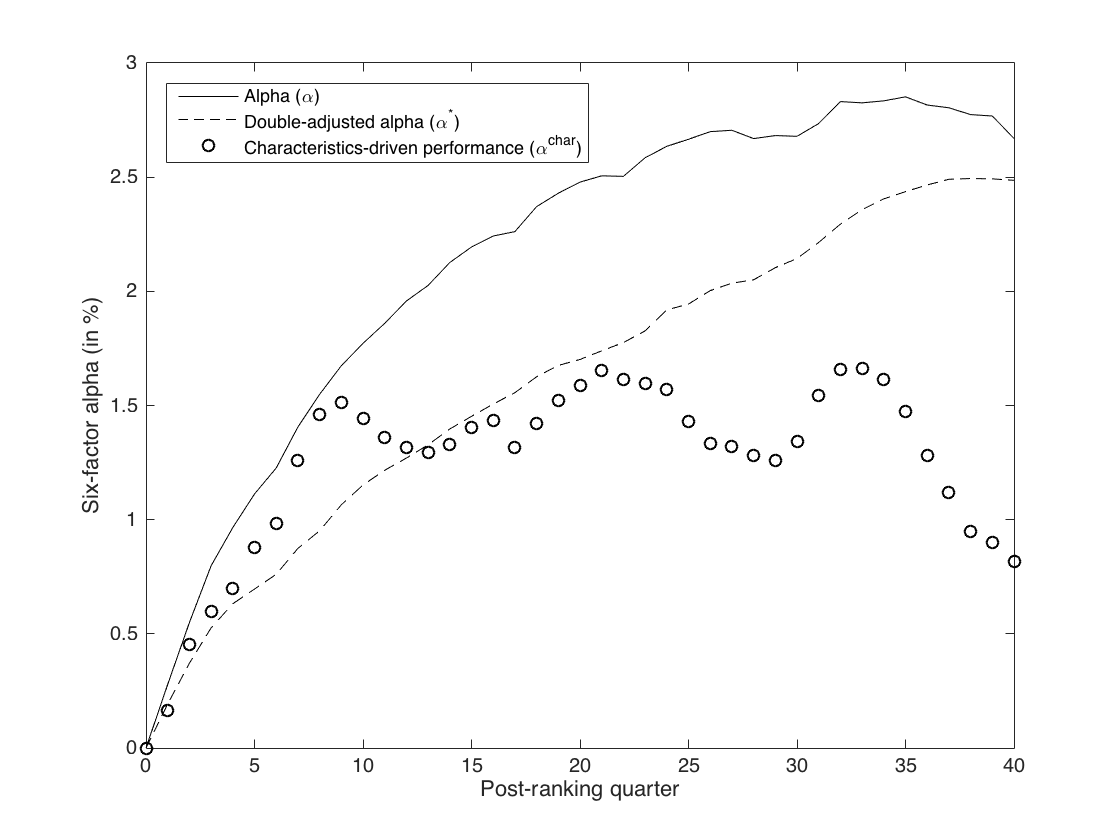
\includegraphics[width=14cm,height=7cm,\textwidth]{pictures/persistence.png}
%   {\captionsetup{justification=centering,singlelinecheck=off}
%   \caption{\bfseries Cumulative alphas for top-minus-bottom portfolios } } }  
% \caption*{This figure presents the cumulative post-ranking Fama-French six-factor alpha for top-minus-bottom portfolios sorted on one of the following performance measures: six-factor alpha ($\alpha$), double-adjusted six-factor alpha ($\alpha^*$), or characteristic-driven performance ($\alpha^{char}$). These performance measures are calculated using rolling windows with a window size of 24 months (see section \ref{double_alpha}). Portfolios are rebalanced every quarter-end and held up to 40 quarters. The horizontal axis shows the post-ranking holding period in quarters.}
% \end{figure}
% \end{singlespacing}


\subsection{Mutual Fund's R-squared}
 Recent studies show that fund performance is positively affected by fund selectivity or active fund management, which is measured by the deviation of fund holdings from a diversified benchmark portfolio. This selectivity measure requires data on the holdings of funds and knowledge on the benchmark indices of funds, which are difficult to obtain. In addition, the benchmark portfolio is not always accurately defined. \citet{amihud2013mutual} propose a simple and intuitive measure of mutual fund selectivity:\footnote{\citet{amihud2013mutual} define fund selectivity as 1 - $R^2$ = $\frac{\text{RMSE}^2}{\text{TotalVariance}}$ = $\frac{\text{RMSE}^2}{\text{SystemeticRisk}+\text{RMSE}^2}$. \newline RMSE is the idiosyncratic volatility, which is the volatility of the factor model residuals. SystemeticRisk is the return variance that is due to the risk factors. Fund selectivity is greater if the fund's idiosyncratic volatility is higher relative to its total variance, meaning that the fund's volatility is less driven by factor-based (systematic) volatility.  } the fund's R-squared ($R^2$), the proportion of the return variance that is explained by the benchmark portfolios, estimated from a multi-factor model. \citet{amihud2013mutual} hypothesize that a low $R^2$ corresponds to high stock selectivity, as a low $R^2$ indicates that mutual returns are not well explained by the Fama-French risk factors. In this respect, they find that $R^2$ has a negative and significant predictive effect on fund performance. 
We replicate the work of \citet{amihud2013mutual} by examining the relation between a fund's factor model $R^2$ and fund performance. Each month, we calculate a fund's $R^2$ from a six-factor model over a 24-month estimation period using daily returns. Following \citet{amihud2013mutual}, since the distribution of $R^2$ is negatively skewed, we apply the log transformation of $R^2$: $\tilde{R}^2$ = $\text{log}\left[\frac{\sqrt{R^2}}{(1-\sqrt{R^2})}\right]$. We test whether fund selectivity explains fund performance by the following panel regression
\begin{alignat}{2}
     \label{R2}
     \text{Performance}_{it} = & \hspace{0.1cm} c_{0t} + c_{1t}\tilde{R}^2_{it} + c_{2t}\text{ExpRatio}_{it-1} + c_{3t}\text{Turnover}_{it-1} + c_{4t}\text{log}(\text{TNA})_{it-1} \nonumber \\ 
     &+ c_{5t}
    \text{log}(\text{FundAge})_{it-1} + v_{it},
 \end{alignat}
 where $\text{Performance}_{it}$ refers to fund i's six-factor alpha ($\alpha$), double-adjusted six-factor alpha $(\alpha^{*}$),
or characteristic-driven performance ($\alpha^{char}$), all estimated over a rolling window of 24 months ending in month $t$. We relate fund performance to the contemporaneous log-transformed R-squared, $\tilde{R}^2$, which is measured over the same rolling window period. Lagged control variables are included in the regression comprising $\text{ExpRatio}$, the total expenses divided by a fund's Total Net Assets (TNA); $\text{Turnover}$, defined as the minimum of aggregated sales or aggregated purchases divided by TNA; $\text{TNA}$ in logarithm; and $\text{FundAge}$ in logarithm, computed as the difference in years between the current date and the date the fund was first offered. The model residuals are given by $v_{it}$. We estimate this regression in each month in our sample.
\par Table \ref{table7} reports the averaged cross-sectional regression coefficients along with Fama-MacBeth t-statistics with the \citet{newey1986simple} correction for time series correlation with 12 lags. Firstly, similar to the findings of \citet{amihud2013mutual}, we find that alpha is higher for funds with lower R-squared, that is, funds with high stock selectivity. The control variables yield no significant estimates. When we consider double-adjusted alpha we find no significant relation with $\tilde{R}^2$. However, the results indicate a significant (inverse) relation between the characteristic-driven component of alpha and R-squared, with t-statistics well above two. A potential reason might be that characteristics can help explain fund returns in cases where the Fama-French factors fail to do so, such that we find a strong inverse relation between characteristic-driven performance and R-squared. Thus, we find that inverse relation between alpha and R-squared does not indicate a positive relation between fund performance and fund selectivity, but rather indicates the poor explanatory power of the Fama-French style factor models. This calls into question the use of R-squared as a measure of fund selectivity. 

% \begin{singlespacing}
% \begin{table}[h!]
% \centering
% \small
% \setlength{\tabcolsep}{11pt}
% {\captionsetup{justification=centering,singlelinecheck=off}
% \caption{ \bfseries Relation between mutual fund performance and $R^2$ }}
% \caption*{This table presents the time series averages of monthly cross-sectional regressions of mutual fund performance measures on fund selectivity, measured by the contemporaneous log-transformed R-squared ($\tilde{R}^2$). As (annualized) performance measures we employ six-factor alpha ($\alpha$), double-adjusted six-factor alpha ($\alpha^*$) and characteristic-driven performance ($\alpha^{char}$). These performance measures are calculated using rolling windows with a window size of 24 months (see section \ref{double_alpha}). We estimate the regressions with and without a set of control variables. \citet{fama1973risk} t-statistics with the \citet{newey1986simple} correction of 12 lags are reported in parenthesis. Estimates significant at the 5\% are in bold font. The monthly regressions cover the period February 2001 until December 2016. }
% \label{my-label}
% \begin{tabular}{crrrrrrrr}
% \hline
%             & \multicolumn{2}{c}{$\alpha$} & &  \multicolumn{2}{c}{$\alpha^*$} &  & \multicolumn{2}{c}{$\alpha^{char}$} \\ \hline
% Cnst        & \textbf{4.770}           & \textbf{4.778}           &  & \textbf{-0.518}           & \textbf{-0.540}          &  & \textbf{1.073}            & \textbf{1.110}            \\
%             & (2.01)          & (1.98)          &  & (-2.12)                   & (-2.20)                  &  & (2.76)                    & (2.61)                    \\
% $\tilde{R}2$         & \textbf{-1.148} & \textbf{-1.269} &  & -0.018                    & -0.021                   &  & \textbf{-0.314}           & \textbf{-0.306}           \\
%             & (-2.12)         & (-2.36)         &  & (-1.02)                   & (-1.18)                  &  & (-2.67)                   & (-2.55)                   \\
% ExpRatio    &                 & 8.112           &  &                           & 0.848                    &  &                           & -0.548                    \\
%             &                 & (1.30)          &  &                           & (1.62)                   &  &                           & (-0.37)                   \\
% Turnover    &                 & -0.081          &  &                           & 0.001                    &  &                           & -0.002                    \\
%             &                 & (-1.78)         &  &                           & (0.32)                   &  &                           & (-0.29)                   \\
% Log(TNA)     &                 & -0.014          &  &                           & -0.001                   &  &                           & -0.002                    \\
%             &                 & (-1.07)         &  &                           & (-0.23)                  &  &                           & (-0.45)                   \\
% Log(FundAge) &                 & 0.015           &  &                           & 0.006                    &  &                           & -0.010                    \\
%             &                 & (0.48)          &  &                           & (1.45)                   &  &                           & (-0.60)                   \\ \hline
% \end{tabular}
% \end{table}
% \end{singlespacing}
%  \subsection{Mutual fund's deviation from benchmarks}
% \citet{jiang2014information} is another study which analyses the relation between fund selectivity and fund performance. They measure fund selectivity by computing the deviations of the weights of stocks in a fund's portfolio from those of the fund's benchmark portfolio. A fund's benchmark is determined by comparing the holdings of a fund with the holdings of most commonly used benchmarks and select the one for which the difference between weights are minimized. They indeed find that funds which deviate from benchmarks generate higher alphas than their low-deviation counterparts. 

\subsection{Mutual Fund Flows}
 There is no shortage of literature on mutual fund flows. The first stream of literature (e.g., \citet{warther1995aggregate}, \citet{edelen2001aggregate}, \citet{brown2003investor}) have focused on aggregate fund flows to the equity market, documenting a positive correlation with contemporaneous stock returns. Early works of \citet{ippolito1992consumer}, \citet{gruber1996another} and \citet{sirri1998costly} find that capital flows to and from funds are strongly related to past fund performance. The general consensus is that the flow-performance relation is positive, asymmetric and convex; the inflows generated by positive returns is of greater magnitude than the outflows due to negative returns. The establishment of a convex flow-performance relation is generally robust to different performance measures varying from raw returns to multi-factor model alphas.
 
 More recently, a second stream of literature goes beyond the simple flow-performance relations.\footnote{A mutual fund's investment style is an important source of information to investors. \citet{cooper2005changing} document an increase in fund flows to funds adopting the current hot investment style in their names. They find that these inflows are similar across funds who alter their positions matching their new name and those who do not, suggesting that investors are irrationally influenced by cosmetic effects. \citet{guo2016mutual} use a fund's reported holdings to determine a fund's investment style and find that funds adopting a more volatile implementation of style strategy garner higher inflows.} A recent paper of \citet{barber2016factors} investigate which risk factors are used by investors to adjust raw returns when evaluating fund performance. They run linear regressions of fund flows on fund alphas obtained from several Fama-French factor models and conclude that CAPM alphas are the best predictor of flows among all factor model alphas. In additional analysis, they decompose fund returns into alpha and returns resulting from factor tilts. They conclude that alpha generates the largest flow response, closely followed by a fund's momentum related return, while flows are least sensitive to fund returns traced to market beta. 
 
We aim to replicate the work of \citet{barber2016factors} using our decomposition of traditional alpha. Using fund flows, we investigate whether investors tend toward the double-adjusted component $\alpha^*$ or toward the characteristic-driven component $\alpha^{char}$ when assessing fund managers. For this purpose, we follow the majority of the prior literature on fund flows and calculate net capital flow\footnote{\citet{frazzini2008dumb} and \citet{lou2012flow} correct for fund mergers when calculating fund flows. As fund mergers are quite rare, this study ignores them.} to fund $i$ during month $t$ as 
 
  \begin{equation}
\label{flow}
    \text{flow}_{it} = \frac{\text{TNA}_{it} - \text{TNA}_{it-1}  (1+R_{it})}{\text{TNA}_{it-1}},
\end{equation}
where $\text{TNA}_{it}$ is fund $i$'s total net assets at the end of month $t$ and $\text{R}_{it}$ is the monthly net return of fund $i$ in month $t$.\footnote{ Fund flows are dropped if the percentage difference in TNA in between two months is greater than 200\% or less than -50\%. These extreme flows are rare and are typically related to structural changes within funds, e.g., mergers.} The variable flow reflects the percentage growth of a fund that is due to new investment (under the assumption of dividends being reinvested in the fund).

% \subsubsection*{Pairwise comparison between performance measures}
% First, we are interested in testing whether the decision-making of fund investors are sensitive to double-adjusted alphas relative to alphas. We consider a pairwise comparison between alpha and double-adjusted alpha. To do so, we proceed as follows. Each month $t$, we sort funds into deciles using both performance measures estimated over the past 36 months. Decile 10 contains the best performing funds, and decile 1 contains the worst performing funds. Thus, we end up with a monthly time-series of two decile ranks (for both alpha and double-adjusted alpha) for each fund.  
% \par 
% We conduct the pairwise comparison by estimating the flow-performance relation with the following panel regression using OLS: 
% \begin{equation}
%     \label{flow_decile} 
%     \text{flow}_{it} = b_0+ \sum^{10}_{k=1} \sum^{10}_{l=1} b_{ab} D_{abit-1} + \gamma X_{it} + \epsilon_{it},
% \end{equation}
% where the dependent variable is the monthly fund flow of fund $i$ in month $t$.  $D_{abit-1}$ is a dummy variable which equals one if fund $i$ in month $t$-1 is in decile $a$ based on alpha and decile $b$ based on double-adjusted alpha. To avoid the dummy variable trap, we exclude the dummy variable for $a$ = 5 and $b$ = 5. The matrix $X_{it}$ contains fund-specific control variables, and $\gamma$ is a vector with corresponding coefficient estimates. The control variables include the previous month-end TNA and the mean of monthly flows over the past year. $\epsilon_{it}$ are the model residuals. The coefficients of interest are $b_{ij}$, which represent the percentage flow received by a fund in decile $a$ using alpha and decile $b$ using double-adjusted alpha. To account for time-fixed effects, we estimate this regression with monthly dummy variables. \par We compare the coefficients for which the decile ranks of both performance measures are equal, but in reversed order. For instance, we compare the coefficient estimate for the dummy variable with funds in the top decile for the alpha and the bottom decile for the double-adjusted alpha ($b_{10,1}$), with the coefficient estimate using funds in the bottom decile for alpha and the top decile for double-adjusted alpha ($b_{1,10}$). If investors favor alpha over double-adjusted alpha to assess fund performance, we expect $b_{10,1}$ $>$ $b_{1,10}$; conversely, if investors are more sensitive to double-adjusted alpha, we expect $b_{10,1}$ $<$ $b_{1,10}$. We conduct this head-to-head comparison for all decile rank combinations, totalling 45 comparisons of coefficients. We test the null hypothesis that the summed difference across all comparisons is equal to zero. Moreover, we compute a binomial test statistic to test the null hypothesis that the percentage of positive coefficient differences is equal to 50\%. 
% \par Figure 3 summarizes the results of the pairwise comparison between the performance measures. In the top left plot, we graph the 45 differences in coefficient estimates when we compare standard four-factor alpha to double-adjusted four-factor alpha as a predictor of fund flows. The horizontal axis displays the decile ranks of both performance measures which are compared. For instance, the bar with label "10v9" contains the difference between the coefficient for funds with alpha ranking of 10 and double-adjusted alpha rank of 9. Overall, funds with higher decile rankings using alpha garner more flows than using double-adjusted alpha. The sum of the differences between coefficients is 47 (t = 3.21), while 83\% of the differences are in favor of alpha. We repeat this procedure and compare the two components of alpha: double-adjusted alpha and characteristic-driven performance (see Eqs.(\ref{double_alpha})-(\ref{char})). The right plot in Figure 3 shows a consistent pattern of positive differences, which indicates that fund flows follow double-adjusted alpha rather than the characteristic-driven component. \par As expected, alpha carries more weight in the assessment of fund performance by investors. \citet{barber2016factors} find that CAPM alphas are the best predictor of flows in comparison to the known multi-factor models. In this light, we can not expect investors to perform a second adjustment to alphas when assessing fund performance.
% However, when we decompose alpha we find that double-adjusted alpha is the component which garners the most flows. That is, in aggregate, investors do not allocate capital to abnormal returns related to the characteristic component of alpha. 

\par Similar to \citet{barber2016factors}, we further decompose characteristic-driven performance into alpha related to each individual characteristic. Recall that characteristic-driven performance (see Eq.(\ref{char})) is defined as
\begin{alignat}{2}
\label{char_decomp}
 \alpha^{char}_{it} &= \delta'_{1t}Z_{it-1} \nonumber \\ 
 &= \delta^{\text{Mcap}}_{1t}\text{Mcap}_{it-1}  + \delta^{\text{B/M}}_{1t}\text{B/M}_{it-1} +  \delta^{\text{Mom12}}_{1t}\text{Mom12}_{it-1} + \delta^{\text{Profit}}_{1t}\text{Profit}_{it-1} + 
 \delta^{\text{Invest}}_{1t}\text{Invest}_{it-1} 
\end{alignat}
which is the sum of lagged (standardized) characteristics multiplied by the corresponding cross-sectional premia. With this decomposition, we gauge whether fund flows are distributed differently across the characteristic components of alpha by estimating the following panel regression 
\begin{alignat}{2}
    \label{decomp}
       \text{flow}_{i,t+1:t+12} = & \hspace{0.1cm} c_{0t} + c_{1t} \alpha^*_{it} + c_{2t} [\delta^{\text{Mcap}}_{1t}\text{Mcap}_{it-1}]  + c_{3t} [\delta^{\text{B/M}}_{1t}\text{B/M}_{it}] +  c_{4t}[\delta^{\text{Mom12}}_{1t}\text{Mom12}_{it-1}] \nonumber \\
        &+ c_{5t}[\delta^{\text{Profit}}_{1t}\text{Profit}_{it-1}] + 
 c_{6t}[\delta^{\text{Invest}}_{1t}\text{Invest}_{it-1}]  \nonumber \\ 
 &+ c_{7t}\text{ExpRatio}_{it} + c_{8t}\text{Turnover}_{it} + c_{9t}\text{log}(\text{TNA})_{it} + c_{10t}\text{log}(\text{FundAge})_{it} + v_{it},
\end{alignat}
where the dependent variable is the average monthly fund flow of fund $i$ in the following year. The independent variables include double-adjusted alpha $\alpha^*_{it}$ and alpha related to a fund's size, value, momentum, profitability and investment characteristics (see Eq.(\ref{char_decomp})). We include the same control variables as in Eq.(\ref{R2}). The model residuals are given by $v_{it}$. We estimate this regression at each year-end. We expect that managerial skill attracts fund, such that there is no capital directed towards abnormal return related to known characteristics. That is, we expect that the parameters related to the characteristic components to be indistinguishable from zero. Contrary evidence implies that either investors are not considering known factors when assessing fund performance, or alpha provides an incomplete risk-adjustment for these characteristics.

% \begin{singlespacing}
% \begin{table}[h!]
% \setlength{\tabcolsep}{23pt}
% \centering
% \small
% {\captionsetup{justification=centering,singlelinecheck=off}
% \caption{ \bfseries Response of fund flows to components of alpha }}
% \caption*{This table presents the time series averages of annual cross-sectional regressions of the one-year ahead average of monthly fund flows on double-adjusted six-factor alpha ($\alpha^*$) and characteristic-driven performance ($\alpha^{char}$). These performance measures are calculated using rolling windows with a window size of 24 months (see section \ref{double_alpha}). We also estimate the regressions in which we further decompose $\alpha^{char}$ into alpha related to each individual characteristic. We estimate the regressions with and without a set of control variables. \citet{fama1973risk} t-statistics with the \citet{newey1986simple} correction of 3 lags are reported in parenthesis. Estimates significant at the 5\% are in bold font. We estimate these annual regressions at the end of each year, covering 16 years from 2001 to 2016.}
% \label{my-label}
% \begin{tabular}{crrrr}
% \hline
% Cnst                    & \textbf{0.014} & 0.004          & \textbf{0.014}  & 0.005           \\
%                         & (6.69)         & (0.58)         & (6.48)          & (0.69)          \\
% $\alpha^*$                      & \textbf{4.061} & \textbf{4.044} & \textbf{4.065}  & \textbf{4.047}  \\
%                         & (9.75)         & (9.80)         & (9.75)          & (9.81)          \\
% $\alpha^{char} & \textbf{0.396} & \textbf{0.366} &                 &                 \\
%                         & (2.41)         & (2.16)         &                 &                 \\
% $\delta^{\text{Mcap}}$ $\cdot$ Mcap            &                &                & \textbf{-1.476} & \textbf{-1.455} \\
%                         &                &                & (-2.19)         & (-2.11)         \\
% $\delta^{\text{B/M}}$ $\cdot$ B/M              &                &                & 0.275           & 0.215           \\
%                         &                &                & (0.31)          & (0.24)          \\
% $\delta^{\text{Mom12}}$ $\cdot$ Mom12              &                &                & \textbf{1.778}  & \textbf{1.720}  \\
%                         &                &                & (3.06)          & (2.91)          \\
% $\delta^{\text{Profit}}$ $\cdot$ Profit           &                &                & 0.338           & 0.221           \\
%                         &                &                & (0.37)          & (0.22)          \\
% $\delta^{\text{Invest}}$ $\cdot$ Invest            &                &                & 1.776           & 1.694           \\
%                         &                &                & (0.85)          & (0.87)          \\
% ExpRatio                &                & 0.481          &                 & 0.468           \\
%                         &                & (1.42)         &                 & (1.40)          \\
% Turnover                &                & 0.000          &                 & 0.000           \\
%                         &                & (-0.96)        &                 & (-1.07)         \\
% Log(TNA)                 &                & 0.000          &                 & 0.000           \\
%                         &                & (-0.82)        &                 & (-0.82)         \\
% Log(FundAge)             &                & 0.002          &                 & 0.002           \\
%                         &                & (1.75)         &                 & (1.78)          \\ \hline
% \end{tabular}
% \end{table}
% \end{singlespacing}

% \vspace{-0.45cm}
\par 
Table \ref{table8} reports the cross-sectional regression coefficients averaged across time along with Fama-MacBeth t-statistics with the \citet{newey1986simple} correction for time series correlation with 3 lags. In the first two columns, we specify future fund flows as a linear combination of double-adjusted alpha and characteristic-driven performance, with and without the set of control variables. We find strong positive relations between both performance measures and fund flows, where the double-adjusted component garners the most inflows. Among the set of control variables, we find positive but statistically insignificant coefficients for $\text{ExpRatio}$ and $\text{log}(\text{FundAge})$.
Of interest are the estimated sensitivities of flows to the characteristic components of alpha. Generally, fund returns related to characteristics do not garner the same magnitude of flows as double-adjusted alpha does. The coefficients on the value and profitability characteristics are both statistically and economically insignificant. However, we do find evidence of investors tending to size and momentum characteristics, which yield significant parameter estimates of about half of that of double-adjusted alpha (in absolute value).  Thus, in aggregate, we find that the flow-performance relation is mostly driven by double-adjusted alpha and that investors allocate a portion of their investment toward funds with favourable characteristics in the size and momentum dimensions. 
\par In sum, we have replicated parts of the analysis from several papers on mutual fund performance. First, we find stronger evidence of return persistence when using double-adjusted alpha. Second, we find that the inverse relation between alpha and R-squared is mostly driven by the characteristic-component of alpha. Third, fund flows are more responsive to double-adjusted alpha rather than characteristic-driven performance. These findings show that adjusting alphas for characteristics materially impacts previous findings on mutual fund performance. As our results together with those of \citet{busse2017double} indicate that double-adjusted alpha better reflects true skill, we believe that this performance measure should be used to reassess previous studies and in future studies on mutual fund performance. 